\documentclass[11pt]{article}
\usepackage[margin=2.5cm]{geometry}
\usepackage[T1]{fontenc}
\usepackage{lmodern}
\usepackage{textcomp}
\usepackage{amsmath,amssymb,bm}
\usepackage{graphicx}
\usepackage{booktabs}
\usepackage{xcolor}
\usepackage[authoryear,round]{natbib}
\usepackage[hidelinks]{hyperref}
\usepackage{caption}
\usepackage{placeins}
\captionsetup{font=small,labelfont=bf}
\renewcommand{\thesection}{\Roman{section}}
\renewcommand{\thesubsection}{\Alph{subsection}}
\newcommand{\todo}[1]{\textcolor{red}{\textbf{TODO:} #1}}
\graphicspath{{../figures/}}

\title{Spatial discriminability in reverberant rooms}
\author{Dominic Bassett\\\todo{affiliation, address, e-mail}}
\date{Draft, \today}

\begin{document}
\maketitle

\begin{abstract}
A room changes the cues a listener uses to tell two source directions apart in two ways: it biases their means and it adds variance to the interaural cues. We derive both from the expected binaural cross-spectral matrix in each auditory band and combine them in a Fisher metric over source direction, built from a listener's own head-related transfer functions. Internal noise is a single interaural coherence ceiling, calibrated once on the lateralisation data of Rakerd and Hartmann (2010) ($\rho=0.984$); precedence enters as a recovery of the weight of later arrivals, with a time constant of 5.6~ms fitted to the lead--lag discrimination data of Litovsky and Shinn-Cunningham (2001). Across 163 heads and a diffuse late field, the frontal azimuth threshold rises from $1.6^\circ$ anechoically to $2.3^\circ$, $5.2^\circ$ and $22^\circ$ at 10, 0 and $-10$~dB direct-to-reverberant ratio (DRR). Above about 5~dB the loss comes mainly from noisier interaural cues; below 0~dB, from compression of all cues. Against measured binaural room impulse responses of five rooms, from an office to a large auditorium, a diffuse field at the measured DRR is conservative by a median of 12--18\%, while the measured first 80~ms with a diffuse remainder reproduces the measured metric to 3--4\%: early reflections, not the late field, carry the room-specific part of the loss. In 420 simulated room configurations, the omnidirectional DRR explains 80\% of the variance in acuity loss at a seat and the standard ISO 3382 parameters add five points, but the dependence on source direction is captured only by the local DRR after head filtering. In shoebox analogues of a lecture theatre, an open-plan dining space and a concert hall, the map of acuity over seats follows the seat's DRR, except near walls, where early reflections leave acuity better than the DRR predicts.
\end{abstract}

\section{Introduction}\label{sec:intro}

How finely a listener can tell two source directions apart is usually measured in anechoic conditions, as the minimum audible angle \citep{mills1958}, and most rooms in which people listen are not anechoic. Reverberation degrades localisation \citep{hartmann1983}: it lowers the interaural coherence at the ears \citep{shinn2005}, compresses interaural level differences most for lateral sources \citep{shinn2005}, and reduces sensitivity to interaural time differences (ITDs) in a way that depends on frequency \citep{rakerd2010}. The precedence effect partly protects the direction of the first arrival against later ones \citep{litovsky1999}. What is missing is a quantitative account of how much spatial discriminability a given room leaves a given listener, in every direction, derived from the acoustics rather than fitted to localisation data from that room.

Ideal-observer models of anechoic localisation \citep{reijniers2014,barumerli2023} predict localisation performance from a listener's head-related transfer functions (HRTFs) and a small set of noise constants. In earlier work we expressed the discriminability of such an observer as a Fisher metric over source direction, whose inverse sets threshold ellipses in every direction \citep{bassett2026}. Here we extend that metric to rooms. The room enters only through the expected binaural cross-spectral matrix in each auditory band; from it the cue means, their variances and the metric follow in closed form. The extension adds two parameters to the anechoic observer, each fitted once on published psychophysics and then held fixed: an internal interaural coherence ceiling, and a time constant for the recovery of later arrivals.

Learned localisers trained in reverberant scenes reproduce many features of human localisation \citep{francl2022} but give no closed-form account of where information is lost. Room-acoustic practice describes spatial impression with parameters such as interaural cross-correlation (IACC) and lateral energy fraction (LF) \citep{iso3382}, which were not designed to predict discriminability. The metric makes two questions answerable: which mechanism limits acuity at a given DRR, and whether acuity is redundant with the standard parameters.

Fisher information and the Cram\'er--Rao bound have been used to relate localisation acuity to neural population codes \citep{jenison2000,harper2004}, in anechoic conditions and for single cues. Binaural models that estimate direction in reverberation select the moments when interaural coherence is high \citep{faller2004} or weight interaural phase by its vector strength \citep{dietz2011}; they predict where a source is heard, not how finely two sources can be told apart. Behaviourally, reverberation reduces localisation accuracy in a frequency- and direction-dependent way \citep{hartmann1983,giguere1993}, and lateral low-frequency sources are heard closer to the midline as reverberant energy grows \citep{ihlefeld2011}; neurally, onset-dominated ITD coding in the midbrain keeps directional information robust in reverberation \citep{devore2009}. A targeted search found no treatment that predicts threshold ellipses in every direction from the head's transfer functions and the room's cross-spectra; the closest are the anechoic ideal observers above.

Section~\ref{sec:theory} sets out the observation model, the cue statistics and their consequences. Section~\ref{sec:methods} describes the heads, the psychophysical data used for calibration, the room models and the measured rooms. Section~\ref{sec:results} reports the calibration, the dependence of acuity on DRR and its mechanisms, precedence, image-source and measured rooms, and the comparison with room-acoustic parameters.

\section{Theory}\label{sec:theory}

\subsection{Observation model}
A static source at direction $\theta$ radiates a stationary Gaussian signal of power spectral density $P(f)$. In a room the binaural transfer function is a sum over arrivals $k$ (direct path $k=0$, reflections $k\ge1$) with amplitudes $a_k$, delays $\tau_k$ and arrival directions $\phi_k$, all functions of $\theta$:
\begin{equation}
\bm H(f,\theta)=\sum_k a_k(f)\,e^{-j2\pi f\tau_k}\,\bm h(f,\phi_k),
\end{equation}
where $\bm h=[h_1,h_2]^{\top}$ holds the directional transfer functions (DTFs) of the left and right ears. The auditory system analyses the ear signals in bands $b$ with power responses $|G_b(f)|^2$, and the expected band cross-spectral matrix is
\begin{equation}
\bm R_b(\theta)=\int |G_b|^2 P\,\bm H\bm H^{\mathsf H}\,df=\sum_{k,l}a_ka_l^{*}\int|G_b|^2P\,\bm h_k\bm h_l^{\mathsf H}e^{-j2\pi f(\tau_k-\tau_l)}\,df.
\end{equation}
If $P$, $a_k$ and $\bm h_k$ vary slowly across a fourth-order gammatone band of bandwidth $\beta_b=1.019\,\mathrm{ERB}(f_b)$, the pair $(k,l)$ contributes in proportion to
\begin{equation}
\kappa_b(\Delta\tau)=e^{-s}\big(1+s+\tfrac25s^2+\tfrac1{15}s^3\big),\qquad s=2\pi\beta_b|\Delta\tau|,
\end{equation}
the Fourier transform of $|G_b|^2$, a Mat\'ern-$7/2$ covariance in the delay difference $\Delta\tau=\tau_k-\tau_l$. The kernel falls to one half at $|\Delta\tau|\approx0.45/\mathrm{ERB}(f_b)$: 5.7~ms at 500~Hz, 3.4~ms at 1~kHz and 1.0~ms at 4~kHz. Arrivals closer together than this \emph{coherence window} add coherently within a band and shape the cue means; arrivals further apart add in power and lower the interaural coherence. The boundary between early and late energy is therefore set by the auditory filter, not by a fixed time such as 50 or 80~ms.

When the late field is dense and isotropic its incoherent sum tends to the diffuse-field matrix of the same head, $\bm\Gamma(f)=\int\bm h(f,\phi)\bm h(f,\phi)^{\mathsf H}\,d\phi/4\pi$, and with unit source power and an omnidirectional direct-to-reverberant ratio $\mathrm{DRR}=1/\eta$,
\begin{equation}
\bm R(f,\theta)=\bm h_e(f,\theta)\bm h_e(f,\theta)^{\mathsf H}+\eta\,\bm\Gamma(f),
\label{eq:R}
\end{equation}
with $\bm h_e$ the direct path and the arrivals coherent with it.

\subsection{Cues and internal noise}
The cues are those of the Barumerli observer \citep{barumerli2023}, written as functionals of $\bm R$: the band levels $L_{i,b}=5\log_{10}S_{i,b}$, $S_{i,b}=\int|G_b|^2R_{ii}\,df$, of each ear and their positive gradients over one ERB; the broadband interaural level difference (ILD), $10\log_{10}(\int R_{11}/\int R_{22})$; and the ITD at the peak of the envelope of the low-passed interaural cross-correlation, $|\int L(f)R_{12}(f)e^{j2\pi f\tau}df|$, on the scale of just-noticeable differences of \citet{reijniers2014}.

Internal noise on the interaural cues is modelled as an internal coherence ceiling $\rho$: a cue estimated from signals of coherence $\gamma$ behaves as if their coherence were $\rho\gamma$. Coherence is taken per auditory band, $\gamma_b=R_{12,b}/\sqrt{R_{11,b}R_{22,b}}$, over a 1-ERB gammatone bank from 80~Hz, because a deterministic set of arrivals has unit coherence at every frequency and loses it only by averaging within a band. The Knapp--Carter bound for a delay estimate \citep{knapp1976} and the delta method for the level ratio give the interaural variances relative to their anechoic values $\sigma^2$:
\begin{align}
v_{\mathrm{ITD}}&=\sigma_{\mathrm{ITD}}^2\frac{I(\bm\gamma^{\mathrm{an}})}{I(\bm\gamma)},\qquad I(\bm\gamma)=\sum_bL(f_b)B_b\omega_b^2\frac{\rho^2\gamma_b^2}{1-\rho^2\gamma_b^2},\\
v_{\mathrm{ILD}}&=\sigma_{\mathrm{ILD}}^2\frac{V(\bm R)}{V(\bm R^{\mathrm{an}})},\qquad V(\bm R)=\sum_b\frac1{B_b}\Big[\frac{R_{11,b}^2}{S_1^2}+\frac{R_{22,b}^2}{S_2^2}-\frac{2\rho^2|R_{12,b}|^2}{S_1S_2}\Big],
\end{align}
with $B_b$ the bandwidth, $S_i=\sum_bR_{ii,b}$, and the anechoic reference at the same direction. The monaural cues keep their anechoic variance: the relative fluctuation of a band power depends on the bandwidth--duration product, not on the room. The duration of the stimulus cancels from every ratio, and $\rho$ is the only parameter the room model adds to the anechoic observer.

\subsection{Fisher metric}
For independent Gaussian cues with means $\mu_m(\theta)$ and variances $v_m(\theta)$, the Fisher information about direction is
\begin{equation}
G_{ij}(\theta)=\sum_m\frac{\partial_i\mu_m\,\partial_j\mu_m}{v_m}+\frac12\sum_m\partial_i\log v_m\,\partial_j\log v_m .
\label{eq:G}
\end{equation}
As $\eta\to0$, $\gamma\to1$ and $v_m\to\sigma_m^2$, the second term vanishes and $G$ is the anechoic metric of \citet{bassett2026}. The threshold at $d'=1$ along a unit tangent direction $\bm e$ is $(\bm e^{\top}G\bm e)^{-1/2}$.

\subsection{Consequences of the diffuse model}
Write $D_{i,b}=S^{\mathrm{dir}}_{i,b}/(\eta\Gamma_{ii,b})$ for the \emph{local} DRR of ear $i$ in band $b$, after head filtering. Because $\eta\Gamma_{ii,b}$ does not depend on $\theta$:
\begin{enumerate}
\item \emph{Level compression.} Band-level slopes shrink by $D_{i,b}/(1+D_{i,b})$. Pinna notches and the shadowed ear have the lowest local DRR and lose spectral information first, so elevation acuity is set by the local DRR in the notch bands rather than by the broadband DRR.
\item \emph{ILD compression.} The ILD slope combines the broadband factors $D_i/(1+D_i)$ of the two ears; the far ear's term vanishes first, so ILD is compressed most for lateral sources.
\item \emph{Coherence.} For a median-plane source of a symmetric head, $\gamma=(De^{j\varphi}+\gamma_d)/(D+1)$, with $\gamma_d=\Gamma_{12}/\Gamma_{11}$ the diffuse-field coherence of the head and $\varphi$ the interaural phase of the direct path. At low frequencies coherence stays high but the phase is pulled towards zero; at high frequencies coherence falls as $D/(D+1)$.
\item \emph{Critical DRR.} The ITD variance doubles when $|\gamma|^2=1/(2-\rho^2)$, i.e.\ at a local DRR $D^{*}=|\gamma^{*}|/(1-|\gamma^{*}|)$ for $\gamma_d\approx0$: about 18~dB for $\rho=0.984$.
\end{enumerate}

\subsection{Precedence}
The stationary model has no precedence: for a source and one copy delayed by more than about 1~ms it carries the same information about the source whether it leads or lags (ratio 0.99--1.03 at 2 and 10~ms). We add precedence as a recovery of the weight of an arrival delayed by $D$ after the direct sound, $w(D)=1-e^{-D/T_s}$, applied to its energy. In the image-source rooms each reflection's amplitude is scaled by $\sqrt{w}$ and the late field by $w$ at its onset; measured responses are weighted sample by sample after the direct part.

\section{Methods}\label{sec:methods}

\subsection{Heads}
HRTFs are those of the SONICOM dataset \citep{engel2023} (free-field compensated, minimum phase, 48~kHz, 793 directions from $-45^\circ$ to $90^\circ$ elevation). One subject (P0203) is excluded for corrupted measurements, leaving 163. Responses are band-limited at 15.5~kHz and converted to DTFs by removing the log-average common transfer function between 50~Hz and 18~kHz; spectra are taken on a 4096-point grid. Integrals over the sphere use spherical Voronoi weights. The DRR sweep and the mechanism analysis use all 163 heads; the other experiments use evenly spaced subsets (12 for the image-source rooms, the ITD and lower-cap checks and the estimator check, 7 for the redundancy analysis, 4 for the frozen-reflection check and 2 for the room maps).

\subsection{Cue model and metric}
Monaural band levels use a 1-ERB gammatone bank from 700~Hz to 16~kHz (27 bands); the ITD uses a tenth-order 3-kHz low-pass and a search over $\pm1$~ms in 2-\textmu s steps with parabolic refinement. Anechoic noise constants are those of \citet{bassett2026}: $\sigma_{\mathrm{mon}}=1.25$, $\sigma_{\mathrm{ILD}}=1$ and $\sigma_{\mathrm{ITD}}=0.569$. Cue means and log-variances are fitted on the sphere by real spherical harmonics of order 6 and differentiated along an orthonormal tangent basis. With $\eta=0$ the spectral-domain cues reproduce the time-domain cues of the anechoic model for nine heads: ILD and ITD correlate at 1.000, spectral gradients at 0.86--0.90 with gradient energy within 11\%, $\sqrt{\det G}$ agrees within 5\% and tensor shape to a median affine-invariant distance of 0.12--0.15. Sixteen unit tests check the anechoic limit, the variance laws against Monte Carlo simulation, the Fisher formula, the coherence window, the room models, the processing of measured responses and the frozen-reflection seat model.

\subsection{Calibration data}
\citet{rakerd2010} measured the lateralisation of 1/3-octave noise bands at 225, 715 and 2850~Hz with interaural coherence 0.2--1.0 and level differences removed. Their psychometric functions (72 points) were read from the vector figures of the article and checked against its curve labels by overlay. A single-interval judgement of the sign of an ITD $\Delta t$ is modelled as $\Phi(\Delta t/\sigma_0\sqrt{m(\gamma)})$ with $m(\gamma)=[(1-\rho^2\gamma^2)/\rho^2\gamma^2]/[(1-\rho^2)/\rho^2]$, a scale $\sigma_0$ per band, the waveform coherence for the two lower bands and the envelope coherence $\gamma^2$ for the 2850~Hz band, and a binomial likelihood of 300 judgements per point.

\subsection{Precedence data}
\citet{litovsky2001} measured ITD just-noticeable differences (jnds) of the lead and of the lag of two 1-ms noise bursts under headphones, at delays of 1--15~ms, with the ITD of the other burst roved over $\pm500$~\textmu s, for six listeners. Their Fig.~3 was digitised from the scanned article (78 points) and checked by overlay. The target's ITD is estimated against the other burst, which dilutes its effective coherence within the binaural integration window,
\begin{equation}
\gamma=\frac{a_t}{a_t+a_n\,e^{-D/T_b}},
\end{equation}
with $(a_t,a_n)=(1,w)$ for the lead and $(w,1)$ for the lag, and $\mathrm{jnd}=A_s\sqrt{m(\gamma)}$ with $\rho$ fixed from the calibration and a scale $A_s$ per listener. Log jnds have Gaussian error; jnds at or above the adaptive-track ceiling of 320~\textmu s (26 of 78) are right-censored.

\subsection{Room models}
\paragraph{Diffuse field.} Eq.~\eqref{eq:R} with $\bm h_e=\bm h(\cdot,\theta)$, at DRR from $\infty$ to $-10$~dB.
\paragraph{Image sources.} A shoebox room with one frequency-independent absorption coefficient supplies images to third order \citep{allen1979}, summed coherently, each filtered by the DTF of its arrival direction. The reverberant energy they do not carry is added as the diffuse field of the head, so that the total matches the statistical reverberant energy $16\pi r^2/R$ for room constant $R$ \citep{kuttruff2016}, with at least the statistical energy after the last image order. DTFs at arbitrary directions are interpolated barycentrically on the convex hull of the measured directions after removing each ear's delay; a virtual vertex at the south pole carries the mean of the lowest ring. Interpolation is exact at the measured directions and errs by 0.5~dB and 2.3~\textmu s (median) in leave-one-out tests.
\paragraph{Measured rooms.} The Surrey set \citep{hummersone2010} holds binaural room impulse responses (BRIRs) of a Cortex Mk.2 head and torso simulator in four rooms (Table~\ref{tab:rooms}), for a loudspeaker at 1.5~m and ear height from $-90^\circ$ to $90^\circ$ in $5^\circ$ steps, and pseudo-anechoic responses of the same head. Each response is cut where its 10-ms energy envelope meets the noise floor and split by a window of $[-1,2.5]$~ms about the onset, with a 1-ms raised-cosine fall, into a direct part and its complement. Cross-spectra are formed at the full response length and summed into the bins of the HRTF grid, which preserves the in-band coherence of arrivals; every response of a room is divided by the common transfer function of its direct parts. The direct part is the anechoic reference and agrees with the pseudo-anechoic set to 2--6\% in threshold. Two models replace reverberant energy by the room's own late field, the cross-spectral matrix after 80~ms averaged over the 37 directions, scaled to the measured energy at each direction: the direct part plus this field, and the measured first 80~ms plus this field. The BRAS benchmark \citep{aspoeck2020,brinkmann2021} adds a large auditorium (CR4, 8\,660~m$^3$): BRIRs of the FABIAN head and torso simulator at one seat (MP6), 10~m from five loudspeakers on the stage (LS3--LS7, at $-8.5^\circ$ to $8.5^\circ$), with the head turned on the torso from $-44^\circ$ to $44^\circ$ in $2^\circ$ steps. Turning the head by $\phi$ places a source at azimuth $\theta_0$ at head azimuth $\theta_0-\phi$, so each loudspeaker gives a measured cue field over $88^\circ$, with the torso fixed. These responses are resampled from 44.1 to 48~kHz and processed in the same way, the late field averaged over all orientations and loudspeakers.

With only the horizontal arc measured, information along azimuth is computed by local quadratic regression of the cue means and log-variances over $\pm20^\circ$. On the SONICOM horizontal plane (12 heads) this estimate agrees with the azimuthal information of the order-6 spherical-harmonic metric to a median of 4\% in threshold anechoically and 8--10\% at 10 to 0~dB DRR, and to 5--7\% in the ratio of room to anechoic threshold (Fig.~\ref{fig:e3}h).

\begin{table}[!tbp]
\centering
\caption{Measured rooms \citep{hummersone2010}. $T_{60}$ from the documentation; DRR and $C_{50}$ as computed here (median over directions); late fraction: share of the reverberant energy after 80~ms.}
\label{tab:rooms}
\small
\begin{tabular}{llcccc}
\toprule
Room & Type & $T_{60}$ (s) & DRR (dB) & $C_{50}$ (dB) & Late fraction\\
\midrule
A & office & 0.32 & 6.5 & 17.9 & 0.02\\
B & classroom & 0.47 & 5.9 & 13.2 & 0.08\\
C & lecture theatre & 0.68 & 9.6 & 20.5 & 0.05\\
D & seminar room & 0.89 & 7.4 & 11.7 & 0.18\\
\bottomrule
\end{tabular}
\end{table}

\subsection{Redundancy analysis}
Three shoebox rooms ($5\times4\times3$, $8\times6\times3$ and $14\times10\times5$~m), five absorptions (0.05--0.5), three random listener positions per room, sources at 1~m (ears at 1.2~m) and, in the tallest room, also at 2~m (ears at 1.8~m), seven heads and eight source directions give 3\,360 source--receiver pairs in 420 configurations; every source lies at least 0.3~m inside the room. The metric is computed for the room, with precedence weighting, and for the anechoic case on 176 near-uniform directions above $-45^\circ$ plus the targets, and the acuity loss at a source direction is $\tfrac12\log(\det G_{\mathrm{an}}/\det G)$. DRR, $C_{80}$, LF (5--80~ms, $\cos^2$ weighting), IACC (mean of the 500, 1000 and 2000~Hz octaves) and $T_{60}$ are computed from the same arrivals. Ordinary least squares with folds that leave out whole configurations gives the cross-validated variance explained.

\subsection{Room maps}
A map needs the metric at many seats for one source position. A seat is described by its reflections relative to the direct sound (delay, arrival direction in the listener's frame, and amplitude, broadband or per octave band) and by the energy and onset of the late field, as a shoebox model or a geometric-acoustics path export provides them. The cue field over source direction is built by moving the direct sound and holding the reflections of the actual source fixed. Against image sources recomputed for every source direction (E5 configurations: three rooms, absorption 0.1 and 0.35, two positions, sources at 1~m, four heads, 384 source--receiver pairs), the frozen reflections reproduce the acuity loss with a correlation of 0.994 and are slightly conservative: azimuth thresholds by a median of 4\%, elevation thresholds by 6\% (12--16\% for sources behind). Listeners face the source and the target is the source direction.

\section{Results}\label{sec:results}

\subsection{One coherence ceiling fits all bands}
A single ceiling shared by the three bands fits the lateralisation data of \citet{rakerd2010}: $\rho=0.984$ (approximately 0.978--0.989), with root-mean-square errors of 1.3, 4.2 and 4.8 percentage points (Fig.~\ref{fig:c1}). Separate ceilings per band do not improve the likelihood; the 225~Hz band, tested at coherence 0.85 and 1.0, is the one that constrains $\rho$. The 715~Hz data of a second listener group, not used in the fit, are predicted to 4.0 percentage points. The greater sensitivity of the 225~Hz band to decorrelation, which Rakerd and Hartmann emphasise, is carried by its scale and not by the ceiling: $\sigma_0=48$~\textmu s at 225~Hz against 10~\textmu s at 715~Hz, a ratio of 4.6 where the $\omega^2$ weighting of the Knapp--Carter information predicts 3.2. Near chance the Gaussian model over-predicts performance (74\% against 60\% at coherence 0.2 and 175~\textmu s in the 715~Hz band).

\begin{figure}[!tbp]
\centering
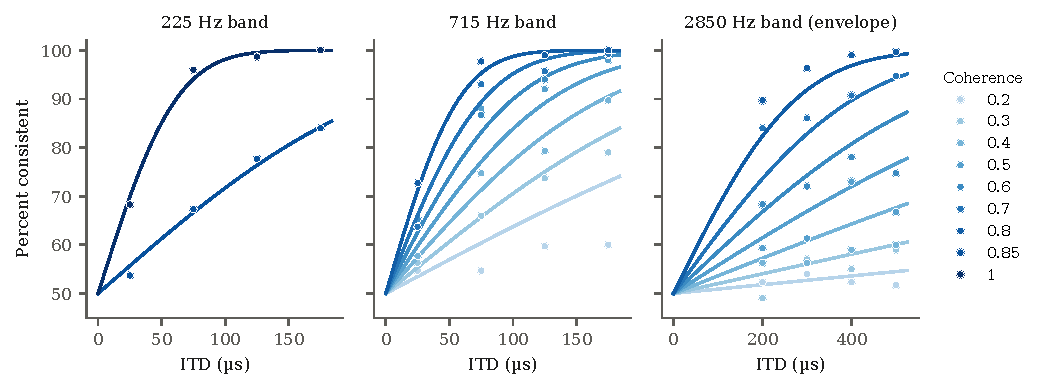
\includegraphics[width=\textwidth]{c1_calibration.pdf}
\caption{Calibration of the internal coherence ceiling on the lateralisation data of \citet{rakerd2010}. Points: proportion of responses consistent with the sign of the ITD; lines: model with one shared ceiling $\rho=0.984$ and a scale per band.}
\label{fig:c1}
\end{figure}

\subsection{Acuity against DRR}
Across all 163 heads, thresholds rise smoothly as DRR falls (Fig.~\ref{fig:e1}). The median frontal azimuth threshold rises from $1.6^\circ$ anechoically to $2.3^\circ$, $5.2^\circ$ and $22^\circ$ at 10, 0 and $-10$~dB ($5.0^\circ$--$5.4^\circ$ at 0~dB over the interval of $\rho$); at $90^\circ$ it rises from $7.3^\circ$ to $9.3^\circ$, $13.9^\circ$ and $40^\circ$. The frontal elevation threshold rises from $4.1^\circ$ to $4.9^\circ$, $8.3^\circ$ and $31^\circ$, almost independently of $\rho$, as level compression predicts. The cues share the information differently as DRR falls: frontally, the ITD carries 33\% anechoically and 7\% at 0~dB, while the spectral cues rise from 14\% to 37\%.

Recomputing the metric with room means and anechoic variances (compression only), and with anechoic means and room variances (inflation only), separates the two mechanisms (all 163 heads). For a frontal source $\sqrt{\det G}$ falls to 0.60 of its anechoic value at 10~dB: 0.84 from compression and 0.72 from inflation, whose product, 0.60, matches the full model. Inflation saturates near 0~dB once the interaural cues have lost their information (0.36--0.75 of anechoic at $-10$~dB, depending on direction), whereas compression keeps falling (0.42 at 0~dB, 0.09 at $-10$~dB). At $90^\circ$ inflation has no effect and the loss is compression alone. Above about 5~dB the room acts mainly by making the interaural cues noisier; below 0~dB, mainly by biasing all cues.

\paragraph{Envelope against fine-structure ITD.} The ITD cue of the Barumerli observer is the peak of the envelope of the cross-correlation below 3~kHz. Replacing it by the peak of the fine structure below 1.5~kHz, with the Knapp--Carter information taken over the same band, changes median azimuth thresholds by at most 4\% at DRRs from 10 to $-10$~dB, at every azimuth (12 heads), and elevation thresholds by less than 1\%; anechoically the change is $-10\%$ to $+8\%$. The fine-structure ITD carries more of the frontal information anechoically (46\% against 42\%) and less in the room (7\% against 13\% at 0~dB). The two estimators are biased in opposite directions by the diffuse field: the envelope peak of a $90^\circ$ source moves outward (from 710 to 747~\textmu s at $-5$~dB and 776~\textmu s at $-10$~dB), because the diffuse cross-correlation is a plateau over the ITDs of the head and the envelope of a plateau peaks at its edges, while the fine-structure peak moves inward (from 716 to 698 and 671~\textmu s), in the direction of the medial bias of lateral low-frequency sources reported by \citet{ihlefeld2011}. Biases do not enter the metric, which depends only on how the cues change with direction. Against the measured rooms, the two models of Sec.~\ref{sec:e3} err by medians of 19\% and 3.5\% with the fine-structure ITD, against 17\% and 2.9\% with the envelope ITD. The envelope ITD is kept, so that the anechoic limit remains the observer of \citet{bassett2026}.

\begin{figure}[!tbp]
\centering
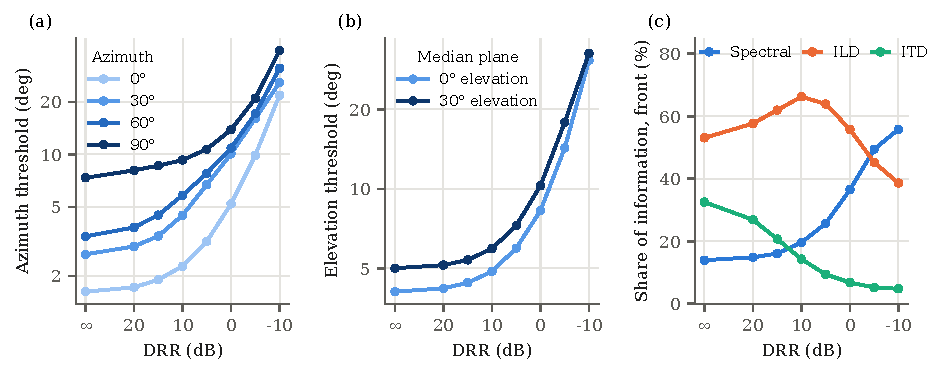
\includegraphics[width=\textwidth]{e1_drr.pdf}
\caption{Median thresholds at $d'=1$ over 163 heads against DRR, direct path plus diffuse field, $\rho=0.984$. (a) Azimuth, horizontal plane. (b) Elevation, median plane. (c) Share of the frontal information carried by each cue family.}
\label{fig:e1}
\end{figure}

\subsection{Precedence}
The weighted model fits the lead--lag jnds with $T_s=5.6$~ms (profile interval 4.6--7.1~ms) and $T_b=50$~ms, a residual standard deviation of 0.28 in log jnd, and is preferred over the stationary model ($w\equiv1$) by an AIC difference of 93 (Fig.~\ref{fig:e2}). The weight of a later arrival recovers to 0.16 at 1~ms, 0.30 at 2~ms and 0.83 at 10~ms. Freeing $\rho$ improves the AIC by 4.6 but drives it to 0.63 and $T_b$ to infinity: the burst experiment constrains the ceiling poorly, and $\rho$ is kept at its calibrated value. The model misses the late recovery of one listener's lag discrimination and the continued rise of lead jnds beyond 10~ms for three listeners.

\begin{figure}[!tbp]
\centering
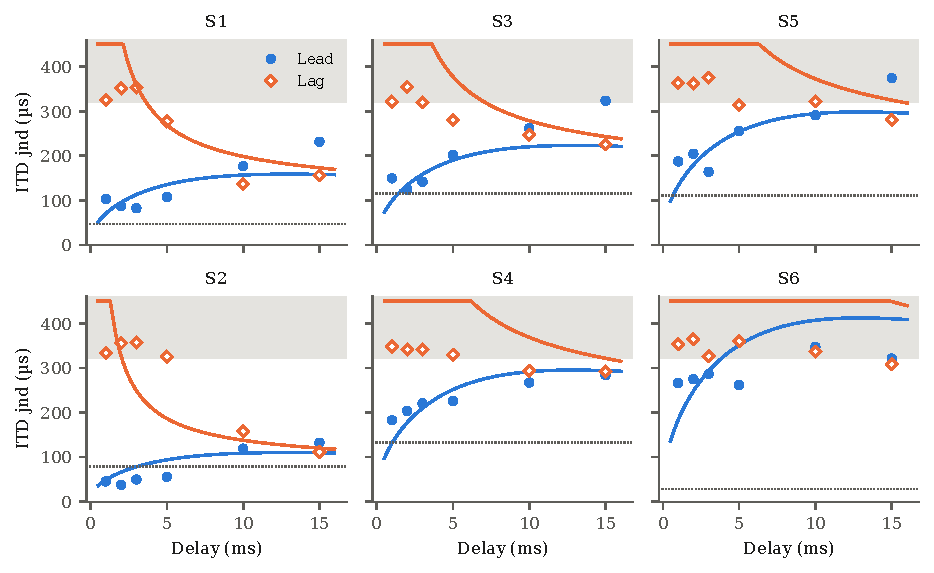
\includegraphics[width=\textwidth]{e2_precedence.pdf}
\caption{ITD jnds of the lead and the lag of two bursts \citep{litovsky2001} against delay, for six listeners, with the weighted model ($T_s=5.6$~ms, $T_b=50$~ms, $\rho=0.984$). Shaded: at or above the adaptive-track ceiling, treated as censored. Dotted: single-burst jnd, not used in the fit.}
\label{fig:e2}
\end{figure}

\subsection{Image-source rooms}
In an $8\times6\times3$~m room with absorption 0.1 and 0.3 (Eyring reverberation times 1.2 and 0.4~s; DRR $-3.1$ and 2.8~dB for a source at 0.9~m), with twelve heads at three listener positions (Fig.~\ref{fig:e1b}):
\begin{itemize}
\item At the same DRR the image-source room degrades acuity less than the diffuse model: frontal azimuth thresholds of $7.1^\circ$ against $8.1^\circ$ at absorption 0.1 and $3.3^\circ$ against $4.1^\circ$ at 0.3. Early images fall within the coherence window of the low bands and keep the ear signals more coherent (frontal band coherence 0.55 against 0.38, and 0.88 against 0.67). The diffuse model is conservative by 10--25\% in threshold.
\item Near a wall and in a corner frontal coherence falls (0.45 against 0.55 at absorption 0.1), as \citet{shinn2005} measured, and frontal thresholds rise modestly ($7.3^\circ$--$7.5^\circ$ against $7.1^\circ$).
\item Precedence weighting changes thresholds by up to $0.4^\circ$, except for sources on the wall side at $90^\circ$, 0.1~m from the wall, whose near-coincident first image it discounts, raising the threshold by $1.1^\circ$--$1.4^\circ$.
\end{itemize}

\begin{figure}[!tbp]
\centering
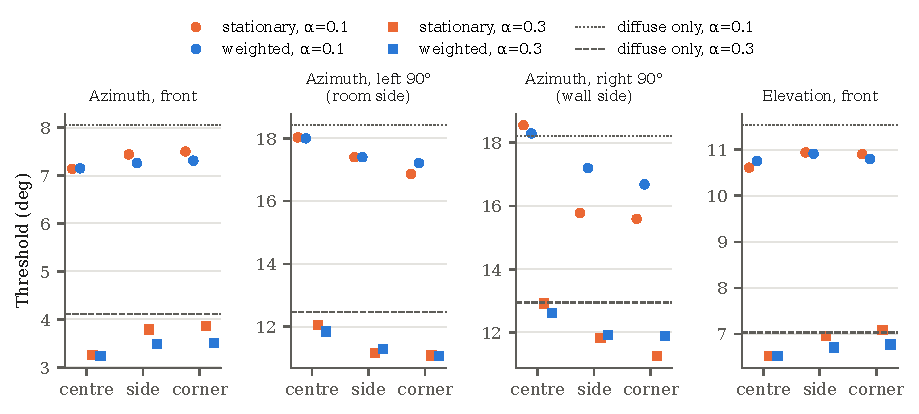
\includegraphics[width=\textwidth]{e1b_shoebox.pdf}
\caption{Median thresholds over twelve heads in an $8\times6\times3$~m image-source room, by listener position, with and without precedence weighting; lines: diffuse model at the same DRR.}
\label{fig:e1b}
\end{figure}

\subsection{Measured rooms}\label{sec:e3}
Reverberation raises the measured azimuth threshold of the head and torso simulator by a median factor of 1.8--2.6 over its direct part (Fig.~\ref{fig:e3}a--d). The direct part plus a diffuse field at the measured DRR, the model of the DRR sweep, over-predicts thresholds at 73\% of directions, by a median of 12\% (median absolute error 17\%). The error is largest at the front (12--41\% by room) and small or reversed laterally ($-9$ to $+25\%$). As in the image-source rooms, measured frontal coherence is higher than the model's (0.75--0.85 against 0.62--0.78): early reflections fall within the coherence window of the low bands.

Keeping the measured first 80~ms and replacing only the remainder by the diffuse field reproduces the measured thresholds to a median of 3\% (90th percentile 9\%; Fig.~\ref{fig:e3}f), with correlations across direction of 0.96--0.99 in log threshold. The late field is therefore well described as a direction-independent field at its measured energy. Its band coherence matches that of a head in an isotropic field (0.56--0.88 at 200~Hz against 0.71 for the SONICOM median; below 0.3 above 500~Hz in both; Fig.~\ref{fig:e3}e), though its level varies with source position by 7--10~dB across the arc. In these rooms only 2--18\% of the reverberant energy at 1.5~m arrives after 80~ms, so most of the loss is carried by early reflections.

Precedence weighting lowers the measured thresholds within $\pm45^\circ$ by 7--12\% and leaves the comparison unchanged (median errors of 13\% and 3\% for the two weighted models); near $\pm60^\circ$, where the measured threshold has a local maximum, it raises them by up to 16\% (Fig.~\ref{fig:e3}g). In the auditorium (Fig.~\ref{fig:e3b}), the seat lies well beyond the critical distance: DRR $-0.9$ to $-3.0$~dB, with 42--51\% of the reverberant energy after 80~ms. Facing each loudspeaker, the measured threshold is $6.5^\circ$--$8.1^\circ$, against $1.8^\circ$--$2.0^\circ$ for the direct part. The same pattern holds as in the smaller rooms: the direct part plus a diffuse field over-predicts the threshold by a median of 18\% (90th percentile 29\%), and the measured first 80~ms plus the diffuse field reproduces it to 3.7\% (90th percentile 10\%), within $\pm24^\circ$ of head turn for all five loudspeakers. Precedence weighting changes these thresholds by about 1\%. This is a test of the room acoustics of the model, not of its psychophysics: no discrimination thresholds have been measured in these rooms.


\begin{figure}[!tbp]
\centering
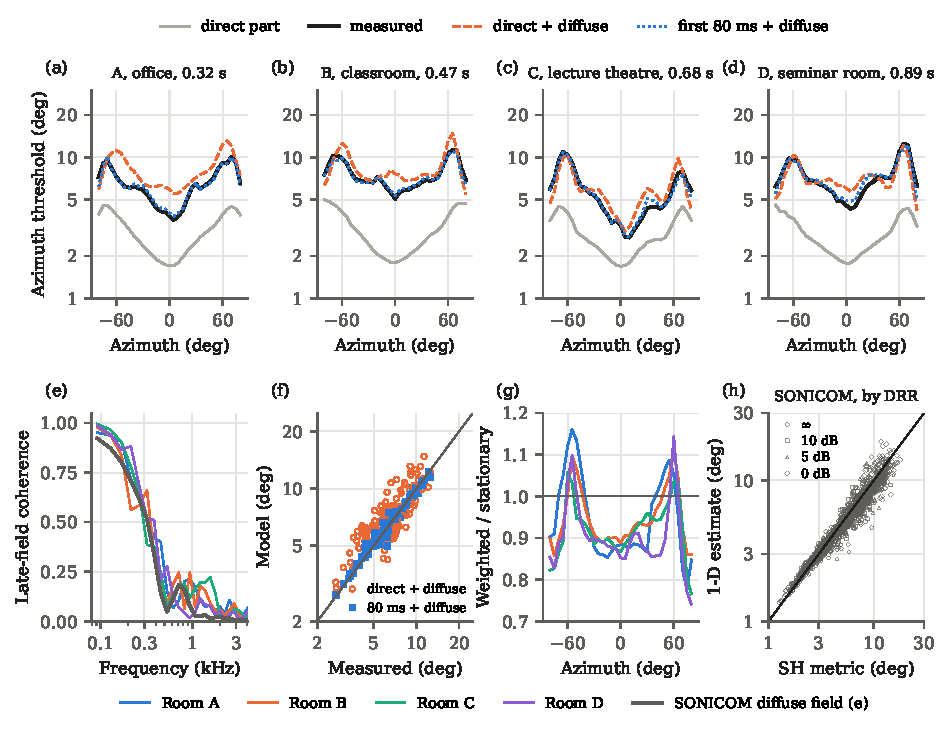
\includegraphics[width=\textwidth]{e3_measured.pdf}
\caption{Measured rooms. (a)--(d) Azimuth threshold at $d'=1$ of the head and torso simulator from its direct part, the measured BRIRs, the direct part plus the room's late field at the measured energy, and the measured first 80~ms plus the late field. (e) Band coherence of the late field (after 80~ms, averaged over directions) and of the SONICOM diffuse field (median of 12 heads). (f) Model against measured thresholds, $|\theta|\le80^\circ$, all rooms. (g) Ratio of precedence-weighted to stationary measured thresholds; room colours as in (e). (h) Check of the 1-D azimuth estimator against the spherical-harmonic metric on the SONICOM horizontal plane, 12 heads.}
\label{fig:e3}
\end{figure}

\begin{figure}[!tbp]
\centering
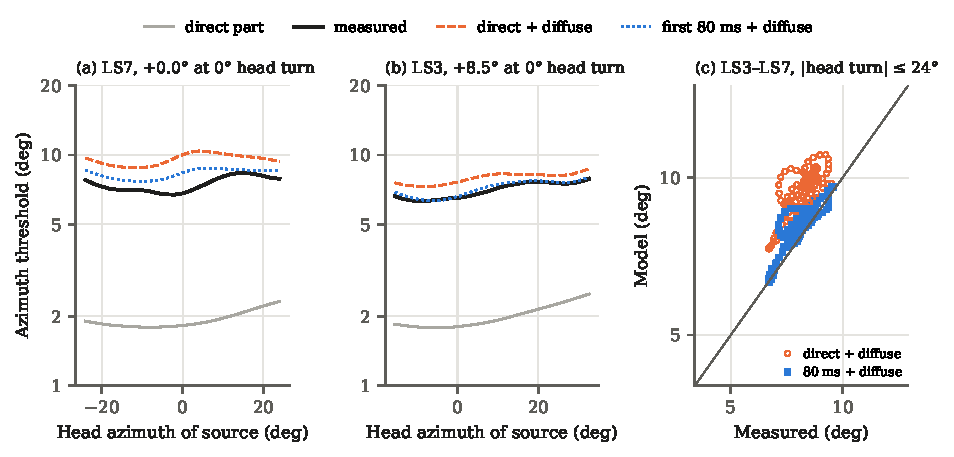
\includegraphics[width=\textwidth]{e3b_cr4.pdf}
\caption{Measured auditorium (BRAS CR4, seat MP6, 10~m from the stage). (a), (b) Azimuth threshold at $d'=1$ of FABIAN against the head azimuth of loudspeakers LS7 and LS3, obtained by turning the head from $-44^\circ$ to $44^\circ$; lines as in Fig.~\ref{fig:e3}. (c) Model against measured thresholds, all five loudspeakers, head turns within $\pm24^\circ$.}
\label{fig:e3b}
\end{figure}

\FloatBarrier
\subsection{Acuity and room-acoustic parameters}
At the level of a seat, the loss of acuity in the simulated rooms is largely redundant with DRR (Table~\ref{tab:e5}, Fig.~\ref{fig:e5}): DRR alone explains 80\% of the cross-validated variance, and $C_{80}$, LF, IACC and $T_{60}$ with their squares and products add five points. What the parameters cannot carry is the dependence on source direction: 18\% of the variance lies across directions within a configuration, and at the same DRR the threshold area grows by a factor of 1.7--2.3 more for sources at $150^\circ$ and $180^\circ$ than at the front, and by 0.6 times as much at $90^\circ$. The head's direct-to-diffuse gain at each direction, which turns the omnidirectional DRR into the local DRR of the theory, accounts for most of that dependence: rear sources are attenuated by the pinna at high frequencies, and a lateral source is boosted at the near ear. The local DRR alone predicts the loss as well as the five standard parameters together, and with them explains 93\%.

\begin{table}[!tbp]
\centering
\caption{Cross-validated variance in acuity loss explained by room-acoustic parameters (3\,360 source--receiver pairs, folds by configuration).}
\label{tab:e5}
\small
\begin{tabular}{lccc}
\toprule
Predictors & Overall & Azimuth & Elevation\\
\midrule
DRR & 0.80 & 0.71 & 0.81\\
DRR, $C_{80}$, LF, IACC, $\log T_{60}$, linear & 0.81 & 0.72 & 0.82\\
the same, with squares and products & 0.85 & 0.77 & 0.85\\
local DRR (DRR plus head gain), with its square & 0.83 & 0.76 & 0.81\\
quadratic set plus head gain & 0.93 & 0.86 & 0.92\\
quadratic set plus source-direction indicators & 0.96 & 0.92 & 0.93\\
\bottomrule
\end{tabular}
\end{table}

\begin{figure}[!tbp]
\centering
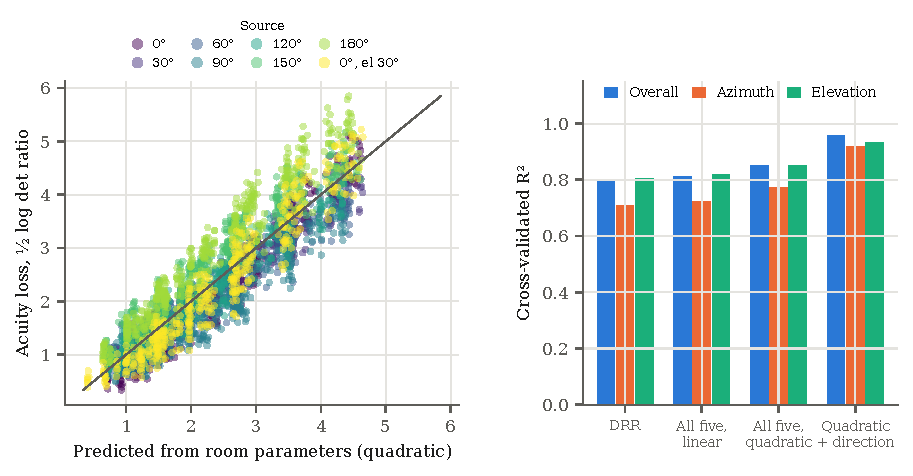
\includegraphics[width=\textwidth]{e5_redundancy.pdf}
\caption{(Left) Acuity loss against its prediction from the five room-acoustic parameters (quadratic model), by source direction. (Right) Cross-validated variance explained by each predictor set.}
\label{fig:e5}
\end{figure}

\subsection{Acuity maps}
Figure~\ref{fig:e6} maps the azimuth and elevation thresholds for the source direction over the seats of shoebox analogues of a lecture theatre ($20\times15\times6$~m, $T_{60}=0.8$~s), an open-plan dining space ($30\times20\times3.5$~m, 1.0~s) and a concert hall ($40\times24\times16$~m, 2.2~s), each with one omnidirectional source, listeners facing it, and two heads. Seat DRRs range from about $-16$ to 0~dB. Azimuth thresholds range from $3.9^\circ$--$5.1^\circ$ at the best seats to $32^\circ$--$40^\circ$ at the worst (anechoic $1.8^\circ$), and stay below $9.4^\circ$ wherever the DRR exceeds $-5$~dB. Elevation thresholds exceed $60^\circ$ at about a third of the seats, where a local threshold no longer describes discrimination.

Within each room the map follows the seat's DRR: a quadratic in DRR explains 96--98\% of the variance of the log-determinant loss across seats. The departure is systematic near walls in the lecture theatre and the concert hall, where the loss is smaller than the DRR predicts (residuals of $-0.17$ and $-0.13$ within 1.5~m of a wall against $+0.08$ and $+0.05$ elsewhere; correlation of residual with wall distance 0.62 and 0.52): a reflection from a nearby wall arrives within a few milliseconds, inside the coherence window and partly discounted by precedence, yet counts as reverberant energy in the DRR. The low dining space shows no such effect. These maps share the limits of the image-source model: uniform absorption, an omnidirectional source and a statistical late field, all of which lower the DRR relative to occupied rooms with directional talkers, and a stationary signal without the onset cues that protect transient sounds.

\todo{repeat the maps for real geometries (a lecture theatre, an open-plan dining space and a concert hall) from geometric-acoustics path exports, e.g.\ from Pachyderm, in the path format of \texttt{sdr/maps.py}, with directional sources and audience absorption.}

\begin{figure}[!tbp]
\centering
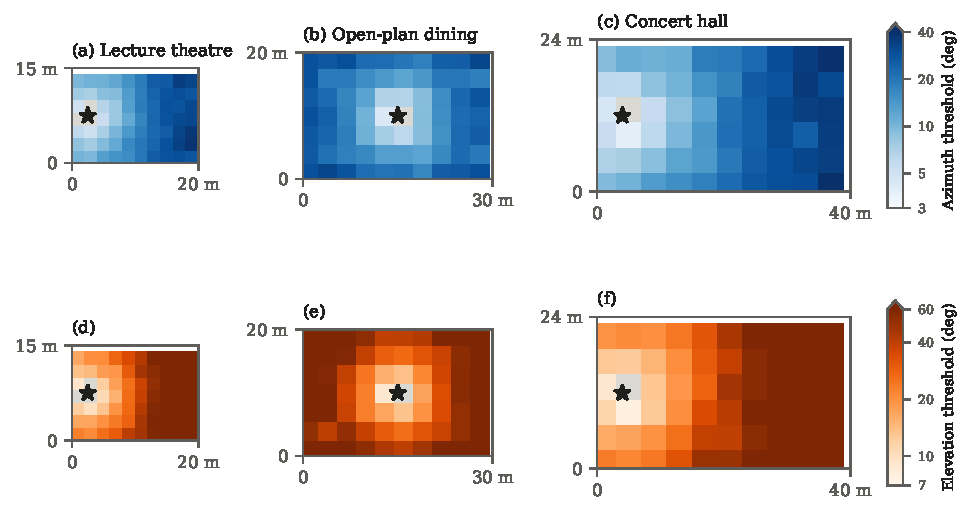
\includegraphics[width=\textwidth]{e6_maps.pdf}
\caption{Acuity maps over seats in shoebox analogues of three room types (plan view; star: source at 1.6 or 1.2~m; ears at 1.2~m; listeners face the source; grey: no seat). (a)--(c) Azimuth and (d)--(f) elevation threshold at $d'=1$ for the source direction, mean of two heads, frozen reflections with precedence weighting. Colour scales are logarithmic and capped at $40^\circ$ and $60^\circ$.}
\label{fig:e6}
\end{figure}

\FloatBarrier
\section{Discussion}\label{sec:discussion}

\subsection{How a room limits acuity}
Two mechanisms combine multiplicatively. At high DRR the room acts on the interaural cues through their variance: coherence falls, the ITD and ILD estimates become noisier, and the ITD's share of the frontal information falls from a third to a few percent by 0~dB. At low DRR the room acts on every cue through its mean: band levels, ILD and the spectral gradients are compressed by the local DRR, and elevation acuity, carried by the spectral cues, follows the local DRR in the notch bands rather than the broadband DRR. The transition lies near 0--5~dB. The measured rooms here, at 5.9--9.6~dB for a source at 1.5~m, lie in the variance-dominated regime; distant seats in larger rooms reach the transition.

\subsection{What the diffuse model gets wrong}
Both the image-source and the measured rooms show the same departure: at a given DRR the diffuse model is conservative by roughly 10--25\%, most at the front, because early reflections arrive within the coherence window of the low bands and keep the ear signals more coherent than a diffuse field of the same energy. The late field itself is well described as diffuse at its measured energy. For prediction, the diffuse model is a bound; for a specific room, the early response must be modelled explicitly and the late remainder can be treated statistically.

\subsection{Relation to room-acoustic parameters}
At the level of a seat, acuity is close to redundant with DRR in shoebox rooms with uniform absorption. Its added value lies in the direction dependence, which no omnidirectional parameter carries and which the local DRR after head filtering does. Shoebox rooms with a statistical late field make the standard parameters strongly correlated with one another (correlation with the loss: DRR $-0.89$, IACC $-0.81$, $C_{80}$ $-0.78$, LF 0.78, $\log T_{60}$ 0.71), which favours redundancy. \todo{repeat the redundancy analysis in rooms with non-uniform absorption, scattering and focusing (geometric-acoustics simulations of real geometries, and measured BRIR sets with full-sphere source positions), before generalising.}

\subsection{Limitations}
The observer is stationary apart from the precedence weighting, and its Gaussian cue model over-predicts performance near chance. The SONICOM grid stops at $-45^\circ$ elevation, so floor reflections from below are approximated by the lowest ring, and in the diffuse-field matrix the Voronoi cells of that ring extend over the unmeasured cap. Filling the cap with mirror images of the directions above $45^\circ$, or giving it no weight, changes median thresholds by at most 2.5\% at DRRs from 10 to $-10$~dB (frontal and $90^\circ$ azimuth, frontal elevation; 12 heads; at most 6\% for any head) and frontal coherence by at most 0.013. The measured rooms cover one head, one distance and the frontal horizontal arc. The predictions are population-level: they use measured HRTFs of many heads and noise constants fitted to other listeners.

\subsection{Behavioural validation}
\todo{A small listening test of azimuth discrimination in measured or rendered rooms at two or three DRRs, with individual HRTFs where available, judged on trends (rank order of conditions, slope against DRR, anisotropy across direction).}

\section{Conclusions}
A Fisher metric over source direction, built from a listener's HRTFs and the expected binaural cross-spectral matrix of a room, predicts how reverberation limits spatial discriminability with two parameters fitted once on published psychophysics. It separates the loss into inflation of interaural variance, dominant above about 5~dB DRR, and compression of all cues, dominant below 0~dB. Against measured rooms, the late field behaves as a diffuse field of the head at its measured energy, and the room-specific part of the loss lies in the early reflections. Acuity at a seat is largely redundant with DRR, but its dependence on source direction requires the local DRR after head filtering. Over the seats of a room, acuity follows the seat's DRR except near walls. \todo{conclusion on maps of real geometries.}

\section*{Acknowledgments}
\todo{acknowledgments and funding.}

\section*{Author declarations}
\todo{conflict of interest statement.}

\section*{Data availability}
Code and derived data: \todo{repository URL}. SONICOM HRTFs: \citet{engel2023}. Surrey BRIRs: \url{https://github.com/IoSR-Surrey/RealRoomBRIRs}. Digitised data of \citet{rakerd2010} and \citet{litovsky2001} are included with the code.

\begin{thebibliography}{99}
\bibitem[Allen and Berkley(1979)]{allen1979} Allen, J.~B., and Berkley, D.~A. (1979). ``Image method for efficiently simulating small-room acoustics,'' J.\ Acoust.\ Soc.\ Am.\ \textbf{65}(4), 943--950.
\bibitem[Asp\"ock et~al.(2020)]{aspoeck2020} Asp\"ock, L., Brinkmann, F., Ackermann, D., Weinzierl, S., and Vorl\"ander, M. (2020). ``BRAS -- Benchmark for Room Acoustical Simulation,'' DepositOnce, Technische Universit\"at Berlin, doi:10.14279/depositonce-6726.3.
\bibitem[Barumerli et~al.(2023)]{barumerli2023} Barumerli, R., Majdak, P., Geronazzo, M., Meijer, D., Avanzini, F., and Baumgartner, R. (2023). ``A Bayesian model for human directional localization of broadband static sound sources,'' Acta Acust.\ \textbf{7}, 12.
\bibitem[Bassett(2026)]{bassett2026} Bassett, D. (2026). ``Evaluating spatial discriminability preservation in HRTF upsampling using Fisher information,'' \todo{venue and status}.
\bibitem[Brinkmann et~al.(2021)]{brinkmann2021} Brinkmann, F., Asp\"ock, L., Ackermann, D., Opdam, R., Vorl\"ander, M., and Weinzierl, S. (2021). ``A benchmark for room acoustical simulation. Concept and database,'' Appl.\ Acoust.\ \textbf{176}, 107867.
\bibitem[Devore et~al.(2009)]{devore2009} Devore, S., Ihlefeld, A., Hancock, K., Shinn-Cunningham, B., and Delgutte, B. (2009). ``Accurate sound localization in reverberant environments is mediated by robust encoding of spatial cues in the auditory midbrain,'' Neuron \textbf{62}(1), 123--134.
\bibitem[Dietz et~al.(2011)]{dietz2011} Dietz, M., Ewert, S.~D., and Hohmann, V. (2011). ``Auditory model based direction estimation of concurrent speakers from binaural signals,'' Speech Commun.\ \textbf{53}(5), 592--605.
\bibitem[Engel et~al.(2023)]{engel2023} Engel, I., Daugintis, R., Vicente, T., Hogg, A.~O.~T., Pauwels, J., Tournier, A.~J., and Picinali, L. (2023). ``The SONICOM HRTF dataset,'' J.\ Audio Eng.\ Soc.\ \textbf{71}(5), 241--253.
\bibitem[Faller and Merimaa(2004)]{faller2004} Faller, C., and Merimaa, J. (2004). ``Source localization in complex listening situations: Selection of binaural cues based on interaural coherence,'' J.\ Acoust.\ Soc.\ Am.\ \textbf{116}(5), 3075--3089.
\bibitem[Francl and McDermott(2022)]{francl2022} Francl, A., and McDermott, J.~H. (2022). ``Deep neural network models of sound localization reveal how perception is adapted to real-world environments,'' Nat.\ Hum.\ Behav.\ \textbf{6}, 111--133.
\bibitem[Gigu\`ere and Abel(1993)]{giguere1993} Gigu\`ere, C., and Abel, S.~M. (1993). ``Sound localization: Effects of reverberation time, speaker array, stimulus frequency, and stimulus rise/decay,'' J.\ Acoust.\ Soc.\ Am.\ \textbf{94}(2), 769--776.
\bibitem[Harper and McAlpine(2004)]{harper2004} Harper, N.~S., and McAlpine, D. (2004). ``Optimal neural population coding of an auditory spatial cue,'' Nature \textbf{430}(7000), 682--686.
\bibitem[Hartmann(1983)]{hartmann1983} Hartmann, W.~M. (1983). ``Localization of sound in rooms,'' J.\ Acoust.\ Soc.\ Am.\ \textbf{74}(5), 1380--1391.
\bibitem[Hummersone et~al.(2010)]{hummersone2010} Hummersone, C., Mason, R., and Brookes, T. (2010). ``Dynamic precedence effect modeling for source separation in reverberant environments,'' IEEE Trans.\ Audio Speech Lang.\ Process.\ \textbf{18}(7), 1867--1871.
\bibitem[Ihlefeld and Shinn-Cunningham(2011)]{ihlefeld2011} Ihlefeld, A., and Shinn-Cunningham, B.~G. (2011). ``Effect of source spectrum on sound localization in an everyday reverberant room,'' J.\ Acoust.\ Soc.\ Am.\ \textbf{130}(1), 324--333.
\bibitem[ISO 3382-1(2009)]{iso3382} ISO 3382-1 (2009). \emph{Acoustics -- Measurement of room acoustic parameters -- Part 1: Performance spaces} (International Organization for Standardization, Geneva).
\bibitem[Jenison(2000)]{jenison2000} Jenison, R.~L. (2000). ``Correlated cortical populations can enhance sound localization performance,'' J.\ Acoust.\ Soc.\ Am.\ \textbf{107}(1), 414--421.
\bibitem[Knapp and Carter(1976)]{knapp1976} Knapp, C.~H., and Carter, G.~C. (1976). ``The generalized correlation method for estimation of time delay,'' IEEE Trans.\ Acoust.\ Speech Signal Process.\ \textbf{24}(4), 320--327.
\bibitem[Kuttruff(2016)]{kuttruff2016} Kuttruff, H. (2016). \emph{Room Acoustics}, 6th ed.\ (CRC Press, Boca Raton, FL).
\bibitem[Litovsky et~al.(1999)]{litovsky1999} Litovsky, R.~Y., Colburn, H.~S., Yost, W.~A., and Guzman, S.~J. (1999). ``The precedence effect,'' J.\ Acoust.\ Soc.\ Am.\ \textbf{106}(4), 1633--1654.
\bibitem[Litovsky and Shinn-Cunningham(2001)]{litovsky2001} Litovsky, R.~Y., and Shinn-Cunningham, B.~G. (2001). ``Investigation of the relationship among three common measures of precedence: Fusion, localization dominance, and discrimination suppression,'' J.\ Acoust.\ Soc.\ Am.\ \textbf{109}(1), 346--358.
\bibitem[Mills(1958)]{mills1958} Mills, A.~W. (1958). ``On the minimum audible angle,'' J.\ Acoust.\ Soc.\ Am.\ \textbf{30}(4), 237--246.
\bibitem[Rakerd and Hartmann(2010)]{rakerd2010} Rakerd, B., and Hartmann, W.~M. (2010). ``Localization of sound in rooms. V. Binaural coherence and human sensitivity to interaural time differences in noise,'' J.\ Acoust.\ Soc.\ Am.\ \textbf{128}(5), 3052--3063.
\bibitem[Reijniers et~al.(2014)]{reijniers2014} Reijniers, J., Vanderelst, D., Jin, C., Carlile, S., and Peremans, H. (2014). ``An ideal-observer model of human sound localization,'' Biol.\ Cybern.\ \textbf{108}(2), 169--181.
\bibitem[Shinn-Cunningham et~al.(2005)]{shinn2005} Shinn-Cunningham, B.~G., Kopčo, N., and Martin, T.~J. (2005). ``Localizing nearby sound sources in a classroom: Binaural room impulse responses,'' J.\ Acoust.\ Soc.\ Am.\ \textbf{117}(5), 3100--3115.
\end{thebibliography}

\end{document}
